
\renewcommand{\arraystretch}{1.3}
\newcommand{\dollar}{\$}
\renewcommand{\kHz}{\si{\kHz}\xspace}
\renewcommand{\MHz}{\si{\MHz}\xspace}
\renewcommand{\W}{\si{\W}\xspace}
\renewcommand{\s}{\si{\s}\xspace}
\newcommand{\Oppers}{~\si[per-mode=symbol]{Op\per\s}\xspace}

\frame{\frametitle{Table of contents}\tableofcontents} 

\section{Objectives}
%\addtocounter{section}{1}


\frame{\frametitle{Objectives}
\begin{itemize}
\item Target: Embedded applications 
\begin{itemize} \item Compound metric: \texttt{P$\times$BS} \end{itemize}
\item Poor Mul/Div execution time
\begin{itemize} \item Implementation with different algorithms \end{itemize}
\end{itemize}
}

\section{Multiplier}
\frame{\frametitle{Multiplier: Wallace Tree}
Algorithm:
\begin{enumerate}
\item Initial \texttt{AND}ing between inputs.
\item Reduce tree using Full Adders and Half Adders.
\item Add the two remaining numbers with a traditional adder.
\end{enumerate}
}

\frame{\frametitle{Pros and Cons}
\begin{columns}
\begin{column}{0.40\textwidth}
\begin{problock}{Pros}
\begin{itemize}
\item Speed improvement.
\item Regular structure.
\end{itemize}
\end{problock}
\end{column}

\begin{column}{0.45\textwidth}
\begin{conblock}{Cons}
\begin{itemize}
\item Resource usage is high.
\item Signifcant Area footprint.
\item Increase in power.
\end{itemize}
\end{conblock}
\end{column}
\end{columns}
}

\frame{\frametitle{Implementation Details}
3 Input Signals:\texttt{RST}, \texttt{CLK} and \texttt{MULI}\\
1 Output Signal:\texttt{MULO}\\
4 generics: \texttt{infer}, \texttt{multype}, \texttt{pipe} and \texttt{mac}

Constants used: WallaceTree (3D logic vector), stages, FA, HA, CIN and RE.
}

\frame{\frametitle{Implementation Details II}
For negative operation - Alternative Baugh Wooley
Negate AND operations (when includes MSD from op1 or op2 but not both)
Add a constant vector at the end.
}

\frame{\frametitle{Implementation Details III}
Feed inputs to FOR-GENERATES (with IF-GENERATES)
IF holdn is HIGH update Add the two final numbers with Baugh-Wooley vector (for signed operations) (ready and nready are not used).
Update MULO.(result/ICC).
}

\section{Divider}
\frame{\frametitle{Divider: Which algorithm?}
\begin{table}
\centering
\begin{tabular}{lcc}
Repeated Multiplication	& \color{green!50!black} \bfseries Fast	& \color{red!40!black} \bfseries Area\\
Reciprocation			& \color{green!50!black} \bfseries Fast	& \color{red!40!black} \bfseries Area\\
Array Divider			& \multicolumn{2}{c}{\color{red!40!black} \bfseries No control on physical placing}\\
Radix >8				& \color{green!50!black} \bfseries Fast	& \color{red!40!black} \bfseries Area\\
Radix-4					& \multicolumn{2}{c}{\color{green!50!black} \bfseries Good compromise}\\
\end{tabular}
\end{table}
\vspace{0.5cm}
\begin{center}
\large \bfseries Execution time $\approx \frac{1}{2}$ of the baseline
\end{center}
}

\frame{\frametitle{Divider II}
\begin{figure}
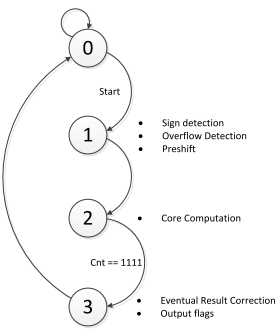
\includegraphics[width=0.9\textwidth,height=0.8\textheight,keepaspectratio]{Figures/DivisorStateMachine.png}
\caption{}
\end{figure}
}

\frame{\frametitle{Divider III}
\begin{figure}
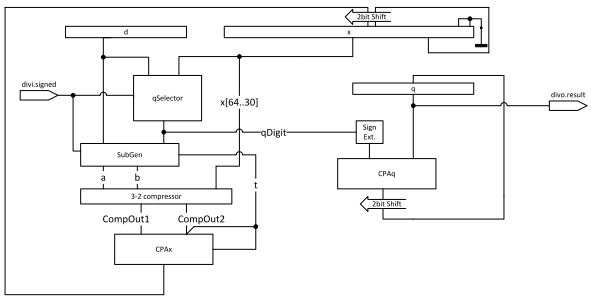
\includegraphics[width=0.9\textwidth,height=0.8\textheight,keepaspectratio]{Figures/DivisorDiagram.png}
\caption{}
\end{figure}
}

\frame{\frametitle{Dvider IV}
\begin{itemize}
\item Signed division (signed p-d plot) vs. Unsigned division (half p-d plot) + 1 cycle for sign
\begin{itemize}
\item No area differences but 1 more cycle delay: signed Division
\end{itemize}
\end{itemize}
}

\frame{\frametitle{Divider V}
\begin{figure}
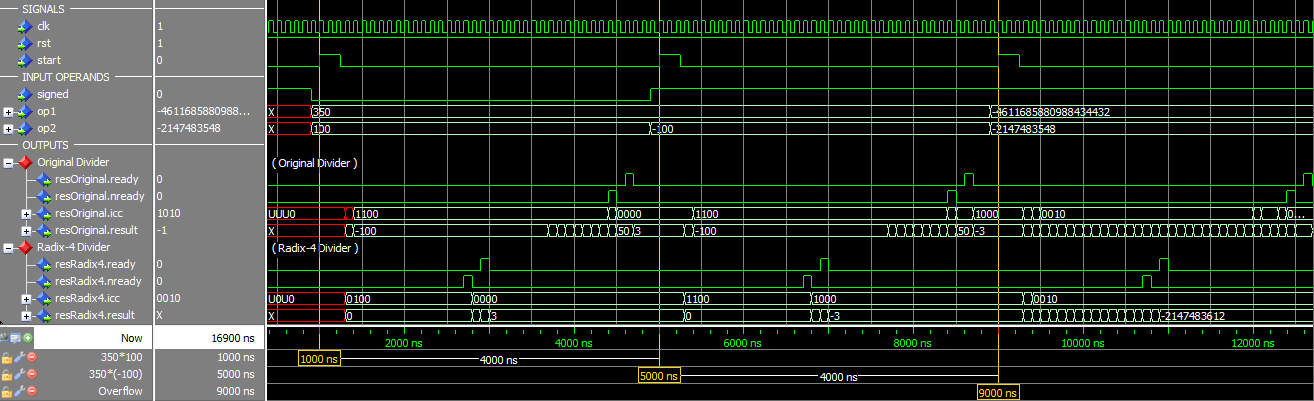
\includegraphics[width=0.9\textwidth,height=0.8\textheight,keepaspectratio]{Figures/myDivisionvsOriginal.png}
\caption{Baseline vs. Radix-4: 19 cycles vs 36}
\end{figure}
}

\section{Synthesis Results}
\frame{\frametitle{Synthesis Results}

\begin{table}[H]
\centering
\begin{tabular}{cccc}
& Baseline & Div & Div\&Mul\\
\midrule
Clock freq. [\MHz]) & 80.522 & 80.535 & 40.197\\
Slices & 9904 & 10479 & 11886\\
LUTs & 16889 & 17865 & 20469\\
Quiescent power [\W] & 2.467 & 2.468 & 2.511\\
Dynamic power [\W] & 0.721 & 0.743 & 0.832\\
Total power [\W] & 3.188 & 3.211 & 3.343\\
P/f [\si[per-mode=symbol]{\W\per\MHz} ] & 0.03959 & 0.03987 & 0.08317\\\toprule
\end{tabular}
\end{table}
}


\section{Benchmarks Scores}
\frame{\frametitle{Benchmarks Scores}
%\fontsize{10pt}{8}\selectfont
\vspace{-.5cm}
\begin{table}[H]
\centering
\begin{tabular}{ccc}
& Baseline & Modified\\
\midrule
Stanford [\s] & 2.30 & 2.21\\
Whetstone [\s] & 116.2 & 112.08\\
Gmpbench Multiply [\Oppers] & 781 & 914\\
Gmpbench Divide [\Oppers] & 15876 & 19205\\
Gmpbench RSA [\Oppers] & 5123 & 5353\\
Division [\s] & 8.06 & 7.31\\
Mibench JPEG (average) [\s] & 23.215 & 21.76\\
SSD [\s] & 10.59 & 8.60\\
Total [\s] & \textbf{219.28} & \textbf{206.92}\\
\toprule
\end{tabular}
\end{table}
%Only slight improvement probably due to the Operating System's Scheduling
}

\section{Conclusion}
\frame{\frametitle{Conclusion - Comparison with Matrics (Div)}

\begin{table}[H]
\centering
\begin{tabular}{cccc}
&Baseline & Modified & Improvements\\\midrule
\ttfamily A & 2.68 & 2.83 & \color{red!40!black} -5.8\%\\
\ttfamily D & 1.24 & 1.24 & - \\
\ttfamily P & 3.19 & 3.21 & \color{red!40!black} -0.7\%\\
\ttfamily BS & 2.19 & 2.13 & \color{green!40!black} 2.7\%\\\midrule
\ttfamily A$\times$D & 3.33 & 3.52 & \color{red!40!black} -5.8\%\\
\ttfamily A$\times$BS & 5.88 & 6.05 & \color{red!40!black} -2.9\%\\
\ttfamily P$\times$D & 3.96 & 3.99 & \color{red!40!black} -0.7\%\\
\ttfamily P$\times$BS & 6.69 & 6.85 & \color{green!40!black} 2.08\%\\
\end{tabular}
\end{table}
}

\frame{\frametitle{Conclusion II - Comparison with Matrics (Div \& Mul)}
\begin{table}[H]
\centering
\begin{tabular}{cccc}
&Baseline & Modified & Improvements\\\midrule
\ttfamily A & 2.68 & 3.24 & \color{red!40!black} -21\%\\
\ttfamily D & 1.24 & 2.49 & \color{red!40!black} -100\%\\
\ttfamily P & 3.19 & 3.34 & \color{red!40!black} -5.0\%\\
\ttfamily BS & 2.19 & 2.07 & \color{green!40!black} 6\%\\\midrule
\ttfamily A$\times$D & 3.33 & 8.05 & \color{red!40!black} -142\%\\
\ttfamily A$\times$BS & 5.88 & 6.69 & \color{red!40!black} -14\%\\
\ttfamily P$\times$D & 3.96 & 8.32 & \color{red!40!black} -100\%\\
\ttfamily P$\times$BS & 6.69 & 6.92 & \color{green!40!black} 1\%\\
\end{tabular}
\end{table}
}

\section{Further Improvements}
\frame{\frametitle{Further Improvements}
\begin{itemize} \item Cache size
	\begin{itemize} \item More power consumption, need to determine actual miss rate
	\end{itemize}

\item Branch prediction
	\begin{itemize} \item Now: Static prediction, only slight advantage, power consumption
	\end{itemize}
	
 \item Out of Order Execution
	\begin{itemize} \item Radical change of the integer unit, improved execution time
	\end{itemize}
	\end{itemize}
}